\documentclass[11pt]{exam}
\usepackage{listings}
\lstset{language=Java}
\usepackage{pdfsync}

\textwidth = 6.5 in
\textheight = 8.5 in
\oddsidemargin = 0.0 in
\evensidemargin = 0.0 in
\topmargin = 0.0 in
\headheight = 0.0 in
\headsep = 0.25 in
\parskip = 0.15in
\parindent = 0.0in

\clubpenalty=10000
\widowpenalty=10000
\sloppy

%\pointsinmargin
%\boxedpoints

%
%  Created by Mike Helmick on 2005-09-26.
%  Copyright (c) 2005 Mike Helmick. All rights reserved.
%
%

\newif\ifpdf
\ifx\pdfoutput\undefined
\pdffalse % we are not running PDFLaTeX
\else
\pdfoutput=1 % we are running PDFLaTeX
\pdftrue
\fi

\ifpdf
\usepackage{subfigure}
\usepackage[pdftex]{graphicx}
\else
\usepackage{graphicx}
\fi

%
%  Update these values for running headers
%
\firstpageheader{\bf\Large Miami University}{\bf\Large EXAM 02}{\bf\Large 03/30/2006 }
\runningheader{CSA274-A Spring 2006}{Miami University}{Exam 02}
\addpoints

\begin{document}

\vspace{3.0in}
\begin{center} 
  \fbox{\fbox{\parbox{5.5in}{\centering
      Miami University - CSA274-A - Spring 2006 - Exam 2 
\par
      There are \numquestions\  questions for a total of  \numpoints\ points.}}}
\end{center} 

% setup standard options for the including code fragments
\lstset{language=Python,numbers=left}

\vspace{0.1in} 
\hbox to \textwidth{Name:\enspace\hrulefill} 

\section*{Instructions}
Please read through this entire exam very carefully before starting.
\par
This exam is closed notes and closed books.
\par
All work must be written on the exam pages in order to be graded.   Any scrap paper used, must be the scrap paper provided during the exam period.
\par
For programming questions: Please be as accurate as possible with your Java syntax: this includes appropriate use of braces, semicolons, and the proper use of upper/lowercase letters.  
\par
A calculator is allowed on this exam.  \newline
No other electronic devices may be used during the exam: this includes iPods, PDAs, and cellular phones.
\par
You have 75 minutes to complete the exam.  
\par
There are \numpoints\ possible points, but the exam will be graded out of 150 points.
\par
{\bf Good Luck!}


\pagebreak

% Questions start here:
\begin{questions}

\section*{Tree Terminology}
\uplevel{Use the tree depicted in this figure to answer the following questions.}
\begin{figure}[htbp]
   \begin{centering}
      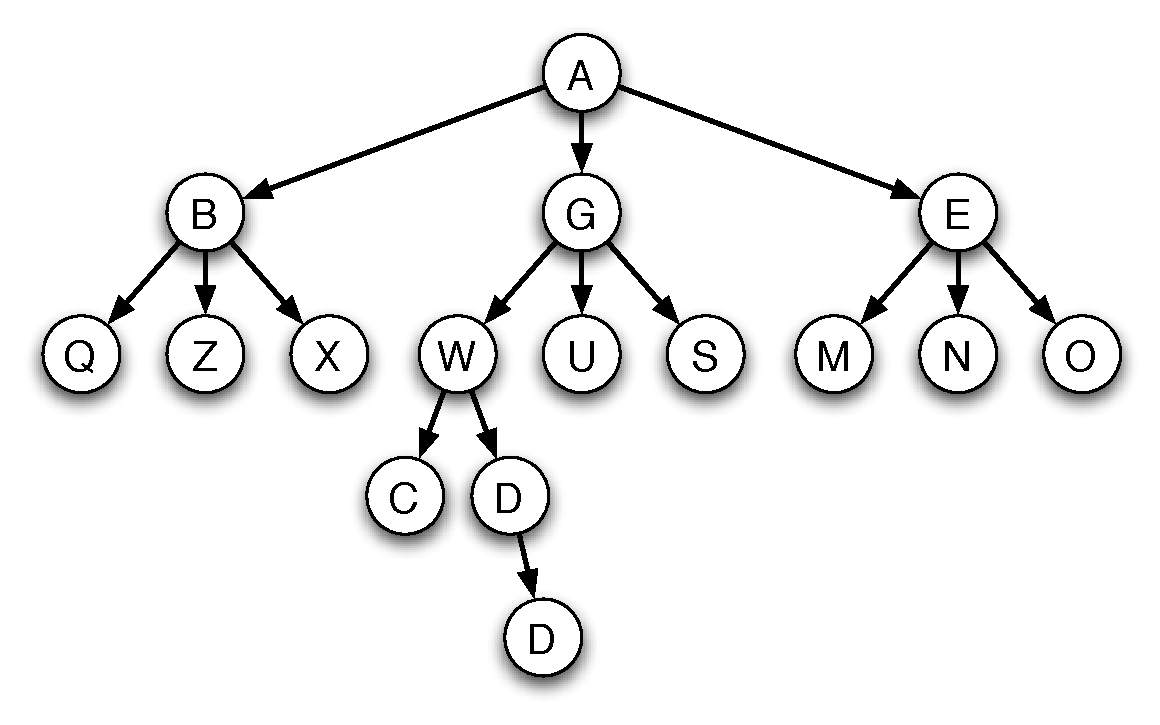
\includegraphics[width=6in]{exam2_tree}
   \end{centering}
   \caption{légende}
   \label{fig:étiquette}
\end{figure}


\question[2] The node labeled A is considered to be the \makebox[1.5in]{\hrulefill} of the tree.
\question[2] This tree has \makebox[2in]{\hrulefill} levels.
\question[2] Node $W$ is at level \makebox[2in]{\hrulefill}.
\question[2] Node $C$ is at level \makebox[2in]{\hrulefill}.
\question[2] Node $B$ has node(s): \makebox[2in]{\hrulefill} as children.
\question[2] (true/false) This tree is a binary tree: \makebox[2in]{\hrulefill}
\question[2] Nodes $Q, Z, M, and N$ are all \makebox[2in]{\hrulefill} nodes.
\question[2] Nodes $B, W, G, and E$ are all \makebox[2in]{\hrulefill} nodes.
\question[2] (true/false) This tree is a full tree: \makebox[2in]{\hrulefill}
\question[2] (true/false) This tree is a complete tree: \makebox[2in]{\hrulefill}

\newpage
\section*{Binary Search Trees}
\question Provide the list correct order for the three steps needed for each type of binary tree traversal
\begin{parts}
   \part[3] Preorder traversal steps
   \begin{enumerate}
      \item \makebox[4in]{\hrulefill} 
      \item \makebox[4in]{\hrulefill} 
      \item \makebox[4in]{\hrulefill} 
   \end{enumerate}
   \part[3] Inorder traversal steps
   \begin{enumerate}
      \item \makebox[4in]{\hrulefill} 
      \item \makebox[4in]{\hrulefill} 
      \item \makebox[4in]{\hrulefill} 
   \end{enumerate}
   \part[3] Postorder traversal steps
   \begin{enumerate}
      \item \makebox[4in]{\hrulefill} 
      \item \makebox[4in]{\hrulefill} 
      \item \makebox[4in]{\hrulefill} 
   \end{enumerate}      
\end{parts}

\newpage

\question[14] Create a binary search tree below, using the numbers provided.   Assign values to the nodes in the tree as if the values are inserted in the order they appear in the list below.
\begin{figure}[htbp]
   \begin{centering}
      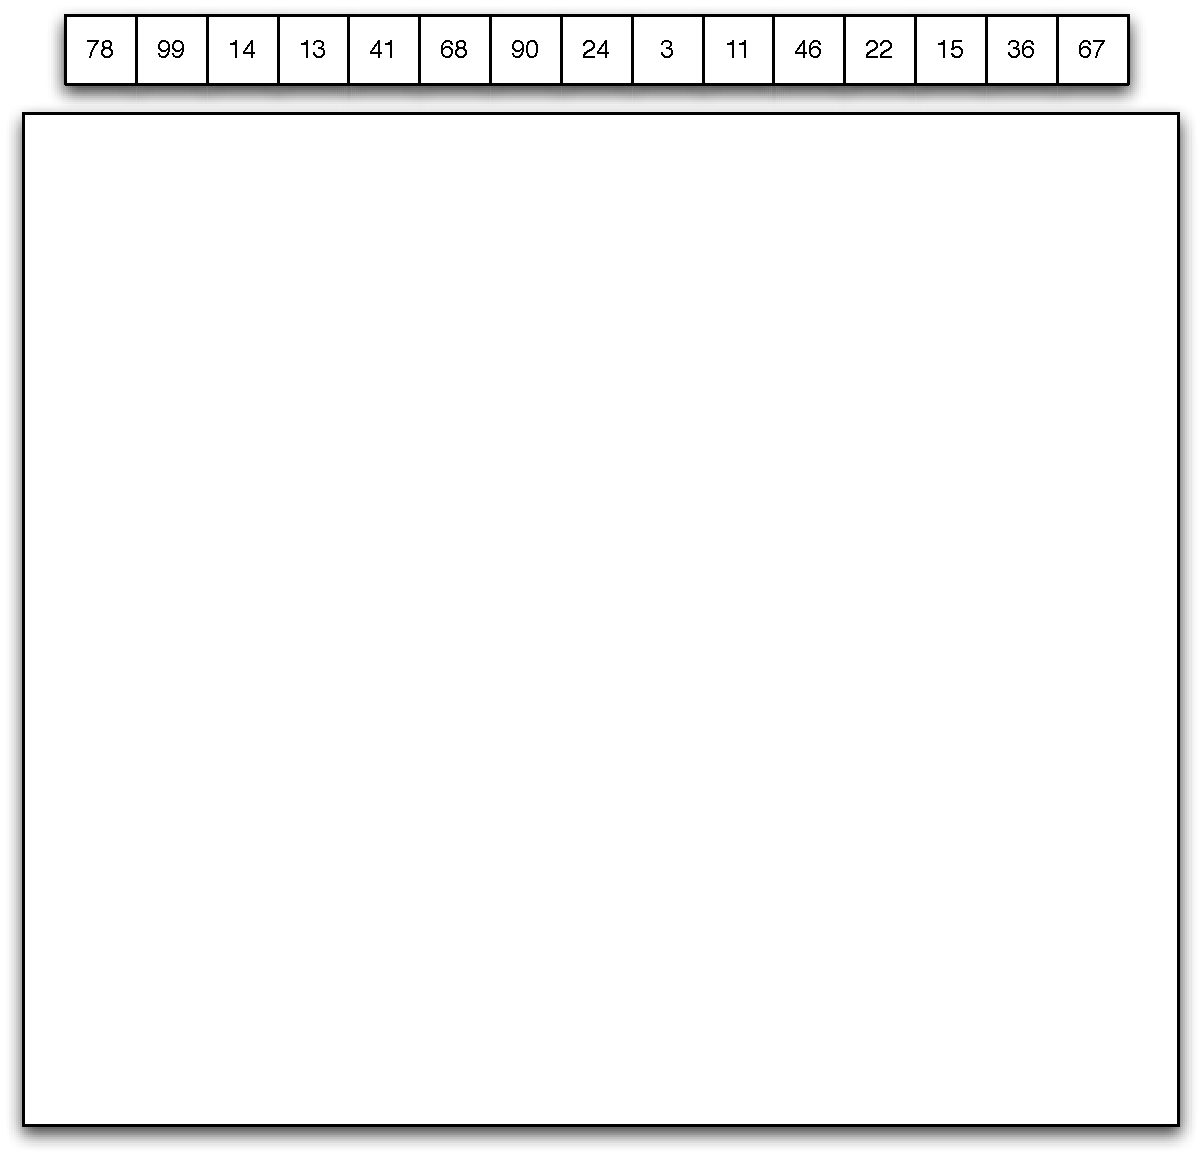
\includegraphics[width=6in]{exam2_binary_search_tree}
   \end{centering}
   \caption{Binary Search Tree}
   \label{fig:bst}
\end{figure}

\question[5] Provide the correct output for a {\bf postorder} traversal on this tree.




\newpage
\section*{Heaps}
\question The largest element in a heap (MaxHeap) must appear in position 0, and the second largest element must be in position 1 or position 2. Give the list of positions (array indices) in a heap of size 15 (array indices zero through 14) where the $k$th largest element (i) can appear, and (ii) cannot appear, for $k = 2, 3, 4$ (assuming the values in the heap are distinct).
\begin{parts}
	\part[5] For $K = 2$
	\vspace{2in}
	\part[5] For $K = 3$
	\vspace{2in}	
	\part[5] For $K = 4$
	\vspace{2in}
	
\end{parts}

\newpage
\question In this question, start with the heap shown in Figure \ref{fig:heap01}.   Follow the instructions for each operation on the heap, showing the status after the operation takes place.   Please proceed with caution as each answer builds on the previous answer.   For operations where there are swaps involved, you should indicate the direction of the swaps with an arrow (the arrow should show the direction of the item being moved).   This is a {\bf MinHeap} over Characters, i.e. maintain alphabetical order $A-Z$.

\begin{figure}[htbp]
   \begin{centering}
      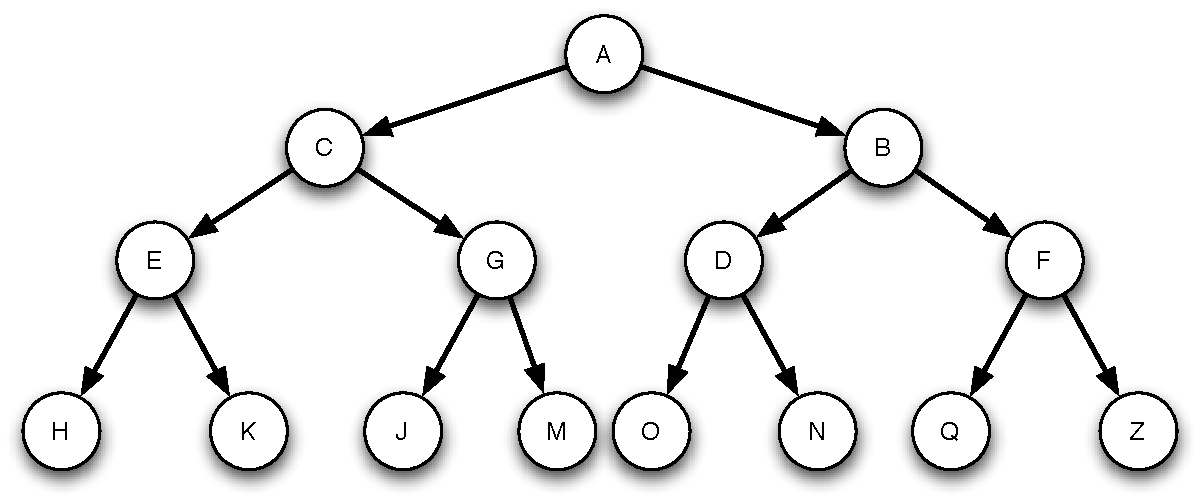
\includegraphics[width=6in]{heap_remove_question_01}
   \end{centering}
   \caption{Starting Heap}
   \label{fig:heap01}
\end{figure}

\begin{parts}
	\part[6] Remove the smallest value from the heap.
	\begin{figure}[htbp]
	   \begin{centering}
	      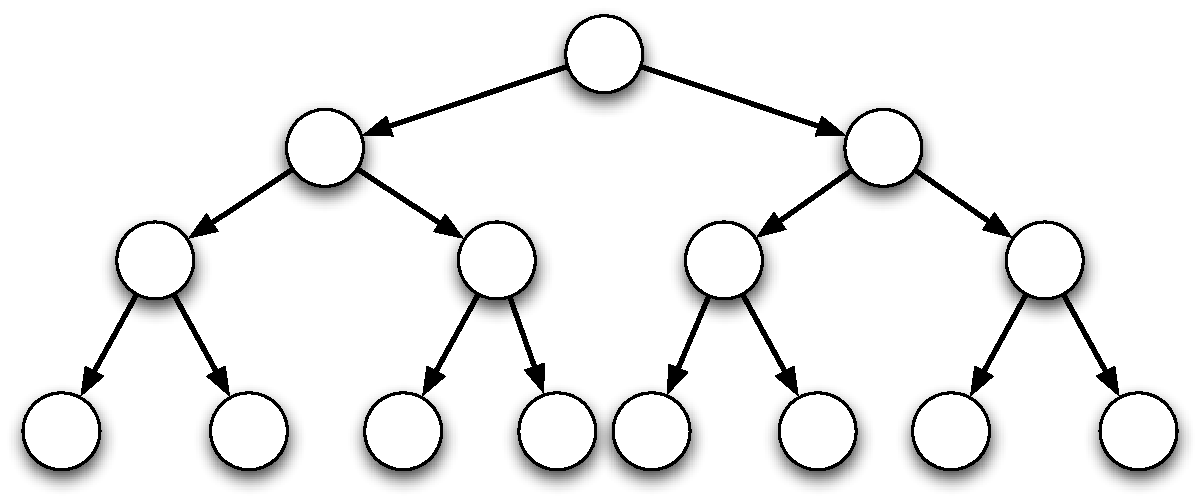
\includegraphics[width=6in]{heap_remove_question_02}
	   \end{centering}
	\end{figure}
\newpage	
    \part[6] Remove the smallest value from the heap.
    \begin{figure}[htbp]
      \begin{centering}
        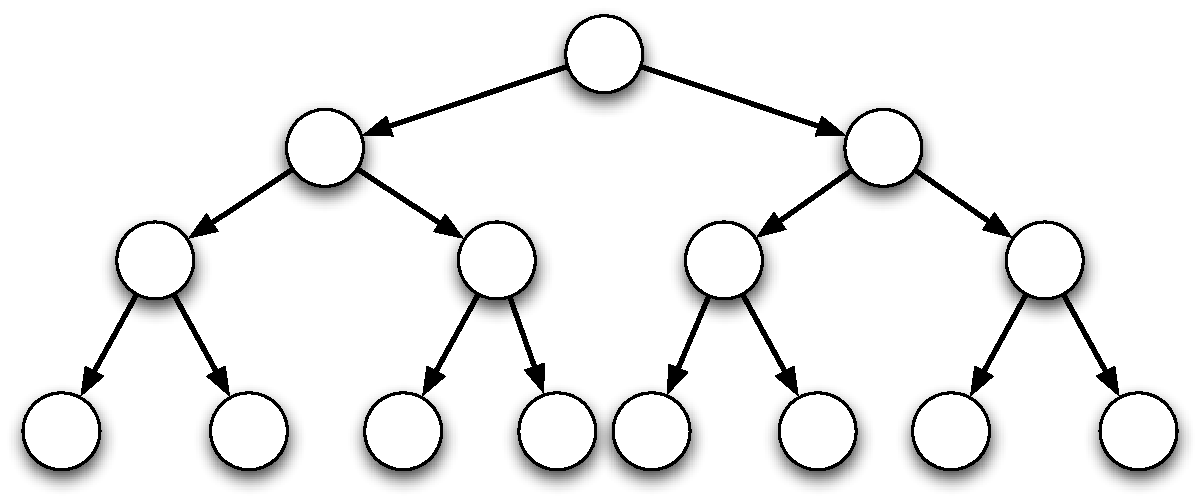
\includegraphics[width=6in]{heap_remove_question_02}
      \end{centering}	
    \end{figure}

	\part[6] Insert the value 'A' into the heap.
	\begin{figure}[htbp]
	  \begin{centering}
	    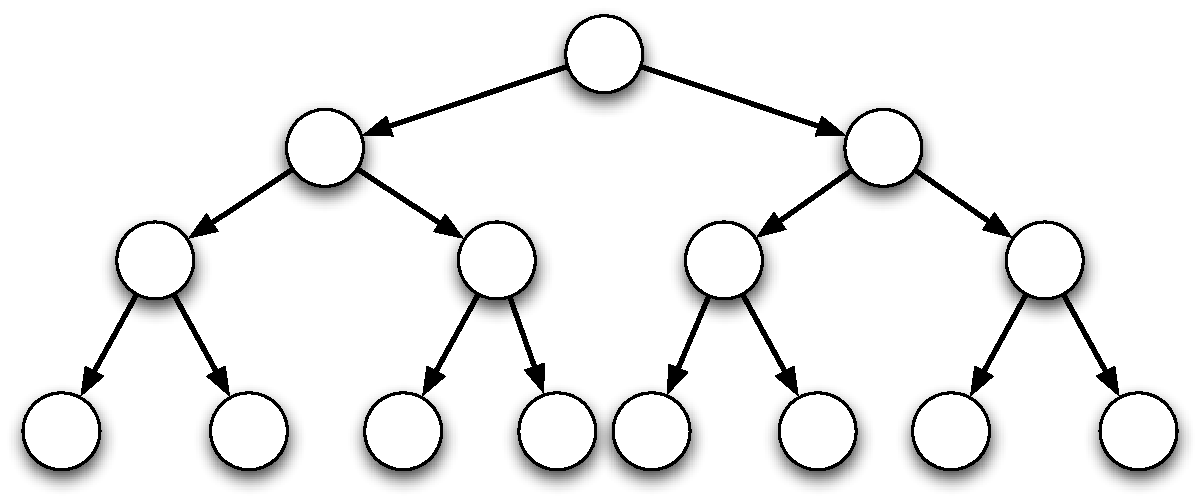
\includegraphics[width=6in]{heap_remove_question_02}
	  \end{centering}	
	\end{figure}
	
    \part[4] Show the array representation of the resultant heap.
	
\end{parts}

\newpage
\section*{Sets, Maps, Hashing}
\uplevel{Fill in the blank.  The following questions pertain to set and map structures, specifically the Java Set and Map interfaces.}

\question[2] (True/False) A set can contain duplicate values: \makebox[2in]{\hrulefill}.
\question[2] Write the line of code for the union operation $a \: \cup \: b$, where you have two Set variables $a$ and $b$.  The result of the union should be stored in set $a$. \newline \makebox[2in]{\hrulefill}
\question[2] Write the line of code for the intersection operation $a \: \cap \: b$, where you have two Set variables $a$ and $b$.  The result of the intersection should be stored in set $a$. \newline \makebox[2in]{\hrulefill}

\question[3] When using open addressing in a hash table, describe the process of removing a key from the hash table.

\vspace{2in}

\question[3] Describe how you can implement a {\tt HashSet} when you have a fully functioning {\tt HashMap} available.

\newpage
\question[18] Show the contents of the hash table that results when you insert items with the keys {\bf E X A M Q U S T I O N} (in this order) into an initially empty hash table of size $M = 16$.   Use the hash function $11k \: mod \: M$, where $k$ is the position of the letter in the alphabet, to determine the hash index of the letter.   Use open addressing with linear probing to handle collisions in the index space.

\begin{figure}[htbp]
  \begin{centering}
    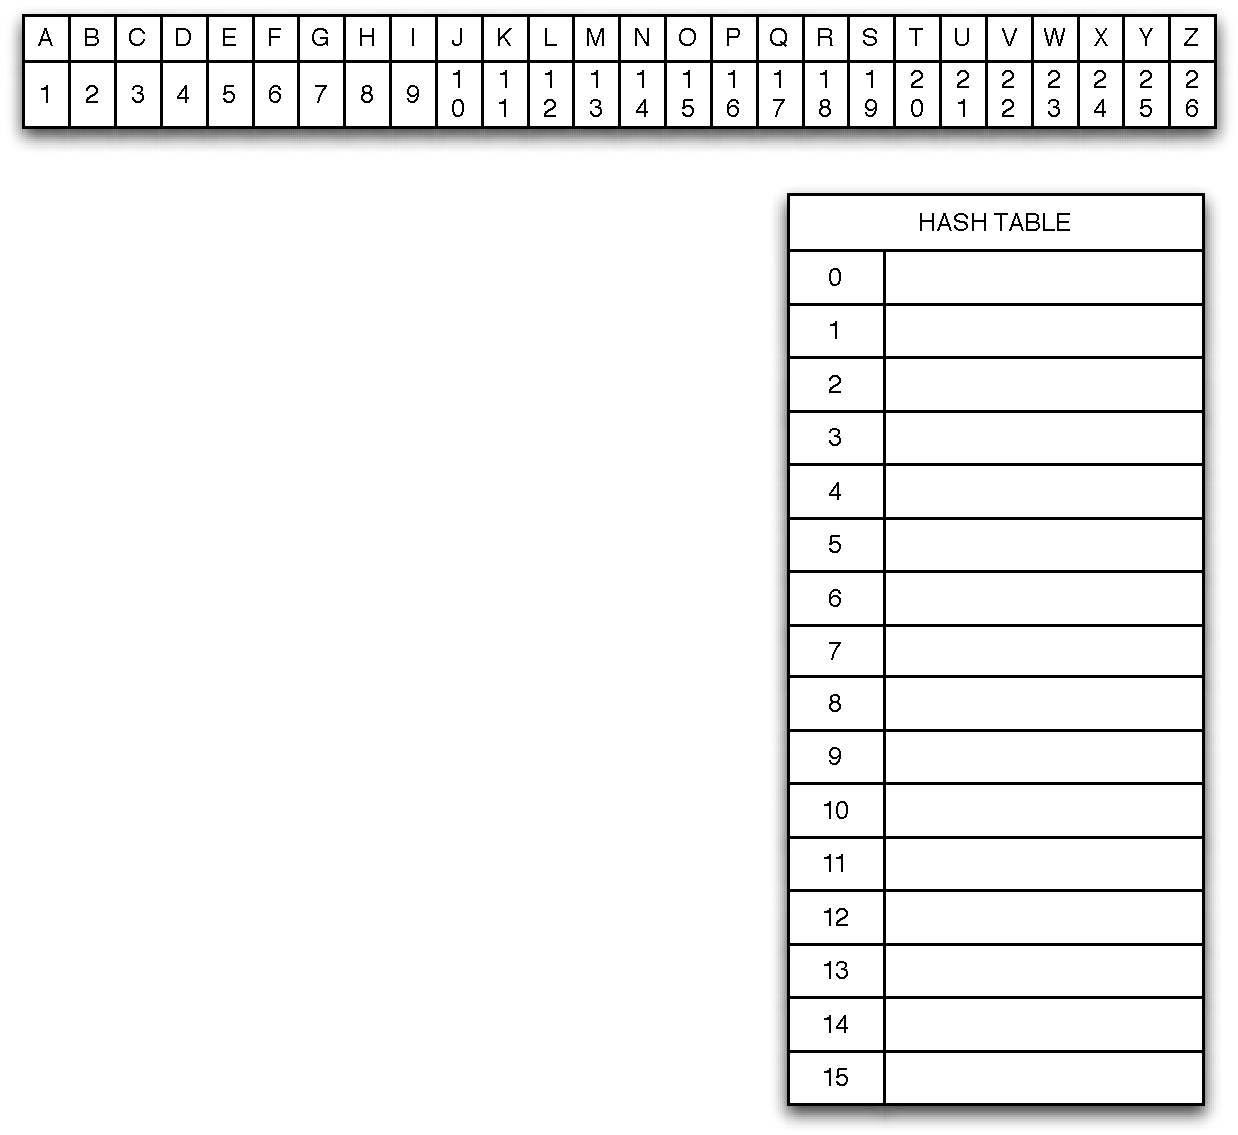
\includegraphics[width=6.5in]{hash_table_question}
  \end{centering}	
\end{figure}

\newpage

\section*{Programming}
\question[18] Code the rehash method for a hash map using open addressing.  You may use the utility methods for which headers have been provided.   You may assume that the rehash method has been invoked because the table is over it's load factor after an add.   Please only use methods and data members that are defined here, as they are necessary and sufficient for solving the problem.

\begin{verbatim}
public class HashMapOpen<K,V> {

  private static final int DEFAULT_SIZE = 101;
  private E[] data = (E[]) new Object[DEFAULT_SIZE];
  private Entry<k,v> DELETED = new Entry<k,v>(null,null);
	
  private int keyCount = 0;
  private int deleteCount = 0;
	
  private static class Entry<K,V> {
    private K key; 
    private V value;
    public Entry( Key k, Value v ) { key = k; value = v }
  }

  public V put( K key, V value ) {
     // implementation details not required
  }
\end{verbatim}	

\uplevel{ {\it your answer goes on the next page} }
\newpage

\begin{verbatim}
  /**
   * The rehash menu at least doubles the capacity of the 
   * internal hash table and reorganizes the table
   * by rehashing the values currently in the table
   *
   * Dummy (deleted) values are removed during this process
   */
  private void rehash() {
	










	
	
	
	
	
	
	
	
	
	
	
	
	
	
	
	
	
	
	
  }
}
	
\end{verbatim}

\newpage
\question[16] For a hash map using chained hashing, implement the {\tt put} method.  The put method must (1) put the new key, value pair in the data array (2) return any previous value that might have been associated with the key (3) check the load factor and call rehash if necessary (just call the rehash method and assume it works).\par
Please assume, that the type $K$ has a working {\tt hashCode} method. 

\begin{verbatim}
public class HashMapChained<K,V> {

  private static final int DEFAULT_SIZE = 101;
  private LinkedList<K,V>[] data = new LinkedList<K,V>[DEFAULT_SIZE];
	
  private int keyCount = 0;
  private final double MAX_LOAD = 3.0;
	
  private static class Entry<K,V> {
    private K key; 
    private V value;
    public Entry( Key k, Value v ) { key = k; value = v }
  }

  private void rehash() { /* call only if the table is aboce MAX_LOAD */ }

  public V put( K key, V value ) {





















  }
\end{verbatim}

\newpage
\question[11] Fill in this recursive method for performing an inorder traversal on this binary search tree class.   When processing a node, simply add it's contents ({\tt data}), plus a space character, to the {\tt StringBuffer} passed in, via the {\tt append} method.

\begin{verbatim}
public class BinarySearchTree<E>
    private Node<E> root;

    private static class Node<E> {
        private E data;
        private Node<E> left;
        private Node<E> right;
        public Node( E data ) { this.data = data }
    }
	
    // rest of the BST implementation omitted
	
    public String printInorder() {
        StringBuffer buf = new StringBuffer();
        printInorder( root, buf );
        return buf.toString();
    }

    private void printInorder( Node<E> localRoot, StringBuffer buffer ) {
	
	
	
	
	
	
	
	
	
	
	
	
	
	
	
	
    }

}
\end{verbatim}


\end{questions}

\end{document}

